\documentclass[tikz]{standalone}
\renewcommand{\familydefault}{\sfdefault}
\begin{document}
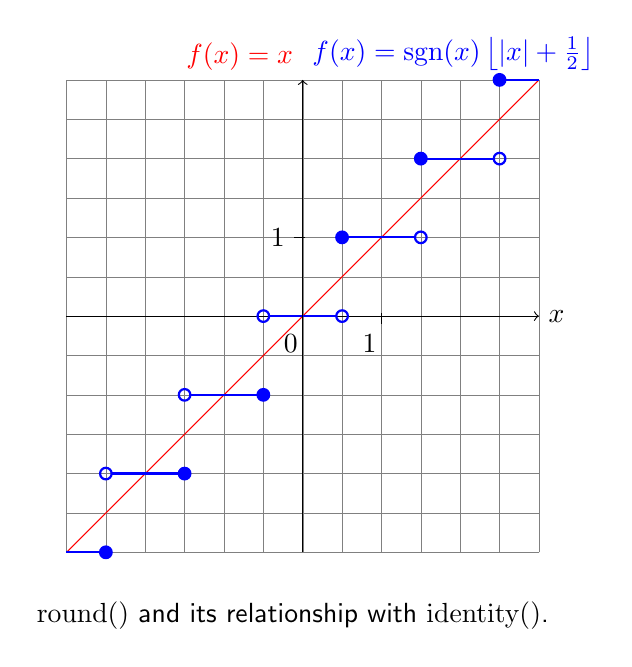
\begin{tikzpicture}
\draw[ultra thin,gray,step=0.5] (-3,-3) grid (3,3);
\draw[help lines] (-3,-3) grid (3,3);
\draw [->][thin] (-3, 0) -- (3, 0) node[right] {$x$};
\draw [->][thin] (0, -3) -- (0, 3) node[above right, blue] {$f(x)= \mathrm{sgn}(x) \left\lfloor \vert x \vert + \frac{1}{2}\right\rfloor$}
node[above left, red] {$f(x) = x$};

\draw [thin, red] (-3, -3) -- (3, 3);

\draw [thick, blue] (-2.5, -3) -- (-3, -3);
\fill [blue] (-2.5, -3) circle [radius=0.0735];
\draw [thick, blue] (-2.5, -3) circle [radius=0.0735];

\draw [thick, blue] (-1.5, -2) -- (-2.4265, -2);
\fill [blue] (-1.5, -2) circle [radius=0.0735];
\draw [thick, blue] (-1.5, -2) circle [radius=0.0735];
\draw [thick, blue] (-2.5, -2) circle [radius=0.0735];

\draw [thick, blue] (-0.5, -1) -- (-1.4265, -1);
\fill [blue] (-0.5, -1) circle [radius=0.0735];
\draw [thick, blue] (-0.5, -1) circle [radius=0.0735];
\draw [thick, blue] (-1.5, -1) circle [radius=0.0735];

\draw [thick, blue] (-0.4265, 0) -- (0.4265, 0);
\draw [thick, blue] (-0.5, 0) circle [radius=0.0735];
\draw [thick, blue] ( 0.5, 0) circle [radius=0.0735];

\draw [thick, blue] (0.5, 1) -- (1.4265, 1);
\fill [blue] (0.5, 1) circle [radius=0.0735];
\draw [thick, blue] (0.5, 1) circle [radius=0.0735];
\draw [thick, blue] (1.5, 1) circle [radius=0.0735];

\draw [thick, blue] (1.5, 2) -- (2.4265, 2);
\fill [blue] (1.5, 2) circle [radius=0.0735];
\draw [thick, blue] (1.5, 2) circle [radius=0.0735];
\draw [thick, blue] (2.5, 2) circle [radius=0.0735];

\draw [thick, blue] (2.5, 3) -- (3, 3);
\fill [blue] (2.5, 3) circle [radius=0.0735];
\draw [thick, blue] (2.5, 3) circle [radius=0.0735];

\foreach \x in {0,1}
\draw (\x cm,1pt) -- (\x cm,-3pt)
    node[anchor=north,xshift=-0.15cm] {$\x$};
\foreach \y/\ytext in {1}
\draw (1pt,\y cm) -- (-3pt,\y cm) node[anchor=east] {$\ytext$};

\node[align=justify, text width=7cm, anchor=north west] at (-3.5, -3.5)
{$\mathrm {round()}$ and its relationship with $\mathrm {identity()}$.};

\end{tikzpicture}
\end{document}